\textbf{\underline{OZ 6 - Magnetische inductie en de wet van Faraday - Oefening 2:}}
\vspace{0.5cm}

    \begin{minipage}{.79\textwidth}
        Een cirkelvormig circuit met straal $r$ bevat een weerstand $R$ en capaciteit $C$, en
        bevindt zich in een uniform magneetveld $\vec{B}$. Startend op tijdstip $t = 0$, begint het spanningsverschil $\Delta V = V_b - V_a$ over de condensator platen toe te nemen met tijd volgens $\Delta V = V_0 (1- e^{\frac{-t}{\tau}})$, met $V_0$ en $\tau$ positieve constanten. Bepaal $\frac{dB}{dt}$, de snelheid waarmee de grootte van het magnetisch veld verandert in functie van de tijd. Wordt $B$ groter of kleiner wanneer de tijd vordert?
    \end{minipage}
    \hspace{0.3cm}\begin{minipage}{.17\textwidth}
        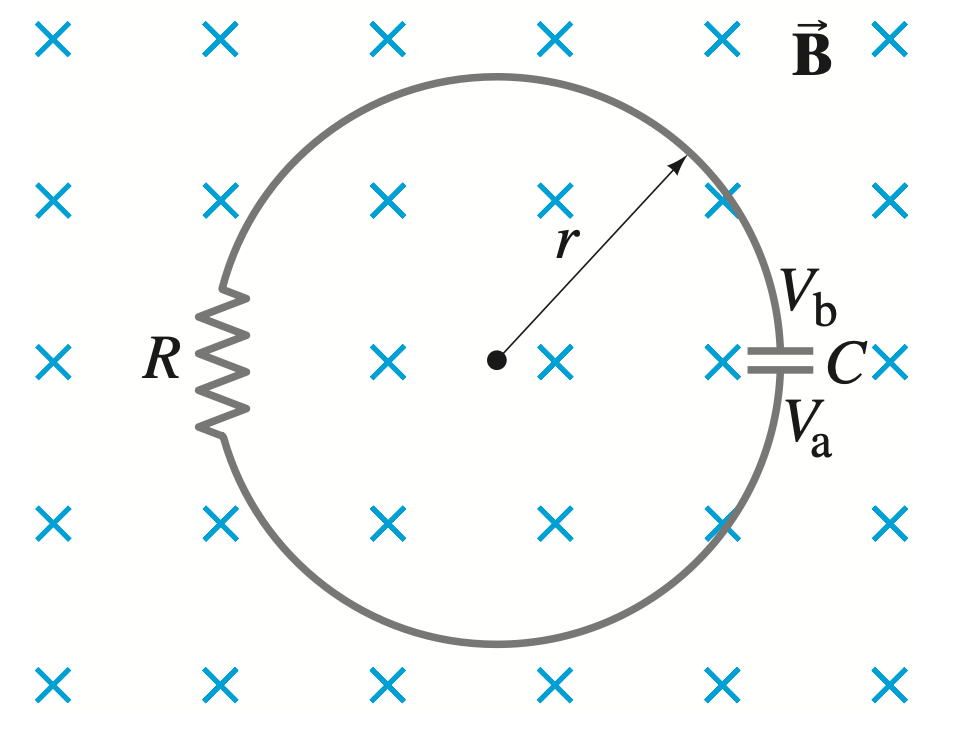
\includegraphics[scale = 0.23]{oz06/resources/Oz6Oef2.png}
    \end{minipage}

    \begin{description}[labelwidth=1.5cm, leftmargin=!]
        \item[Geg. :]
        \item[Gevr. :] 
        \item[Opl. :]
    \end{description}


\vspace{1cm}